%\documentclass{beamer} %voce pode usar este modelo tambem
\documentclass[t,handout,9pt]{beamer}
\usepackage{graphicx}
\usepackage{url}
\usepackage[british]{babel}
\batchmode
% \pgfpagesuselayout{4 on 1}[letterpaper,landscape,border shrink=5mm]
\usepackage{amsmath}
\usepackage{amssymb}
\usepackage{amsfonts}
\usepackage{enumerate}
\usepackage{epsfig}
\usepackage{bbm}
\usepackage{calc}
\usepackage{adjustbox}
\usepackage{color}
\usepackage{ifthen}
\usepackage{capt-of}
\usepackage{float}
\usepackage{booktabs}
\usepackage{dcolumn}
\usepackage{multicol}
\usepackage{hyperref}
\usepackage[flushleft]{threeparttable}
\usepackage{subcaption}
\usepackage{adjustbox}
\usepackage{ragged2e}
\usepackage{xcolor}
\usepackage{pgfpages}
%\usepackage{showframe}

\usepackage{cmbright}

\renewcommand\ttdefault{cmvtt} % selects CM typewriter

\usepackage[utf8]{inputenc} % Required for inputting international characters
\usepackage[T1]{fontenc} 	% Output font encoding for international characters

%\DeclareFontShape{OT1}{cmss}{b}{n}{<->ssub * cmss/bx/n}{}

\usetheme[compress]{Berlin}
\definecolor{sapienza}{RGB}{0, 49, 83}
\usecolortheme[named=sapienza]{structure}

\usepackage[backend=bibtex,style=alphabetic,giveninits=true,url=false,eprint=false,doi=false]{biblatex}
\DeclareNameAlias{sortname}{last-first}
\renewcommand*{\nameyeardelim}{\addcomma\addspace}
\renewcommand*{\bibfont}{\footnotesize}
\addbibresource{example.bib}
\setbeamerfont{footnote}{size=\tiny}

\setbeamerfont{title}{size=\LARGE}

% reduce spaces between tables/figures and caption
\usepackage[font=small,skip=1pt]{caption}

%% pgf plots stuff
%\usepackage{pgfplots}
%\pgfplotsset{compat=newest}
%% the following commands are needed for some matlab2tikz features
%\usetikzlibrary{plotmarks}
%\usetikzlibrary{arrows.meta}
%\usepgfplotslibrary{patchplots}

% one navigation dot per slide trick
\AtBeginSection[]{\subsection{}}

% fix misbehave for allowframebreaks
\usepackage{etoolbox}
\makeatletter
\patchcmd{\slideentry}{\ifnum#2>0}{\ifnum2>0}{}% replace the subsection number test with a test that always returns true
% use frame numbers instead of subsection slide numbers so that frames broken over slides get separate circles
\patchcmd{\slideentry}{\c@subsectionslide}{\c@framenumber}{}{\@error{unable to patch}}
\patchcmd{\beamer@writeslidentry}{\c@subsectionslide}{\c@framenumber}{}{\@error{unable to patch}}

% date in footer trick
\makeatletter
  \setbeamertemplate{footline}{%
    \begin{beamercolorbox}[colsep=1.5pt]{upper separation line foot}
    \end{beamercolorbox}
    \begin{beamercolorbox}[ht=2.5ex,dp=1.125ex,%
      leftskip=.3cm,rightskip=.3cm plus1fil]{author in head/foot}%
      \leavevmode{\usebeamerfont{author in head/foot}\insertshortauthor}%
      \hfill%
      {\usebeamerfont{institute in head/foot}\usebeamercolor[fg]{institute in head/foot}\insertshortinstitute}%
    \end{beamercolorbox}%
    \begin{beamercolorbox}[ht=2.5ex,dp=1.125ex,%
      leftskip=.3cm,rightskip=.3cm plus1fil]{title in head/foot}%
      {\usebeamerfont{title in head/foot}\insertshorttitle\hfill\insertshortdate}%
    \end{beamercolorbox}%
    \begin{beamercolorbox}[colsep=1.5pt]{lower separation line foot}
    \end{beamercolorbox}
  }
\makeatletter

% remove dot for titlepage and Outline
\makeatletter
\let\old@beamer@writeslidentry\beamer@writeslidentry
\def\beamer@writeslidentry{%
  \expandafter\beamer@ifempty\expandafter{\beamer@framestartpage}{}% does not happen normally
  {%else
    \clearpage\beamer@notesactions%
  }
}
\makeatother

% let's number figure captions
\setbeamertemplate{caption}[numbered]

% trick for grouping equations
\newenvironment{rcases}
  {\left.\begin{aligned}}
  {\end{aligned}\right\rbrace}

%-------------------------Titulo/Autores/Orientador------------------------------------------------
\title[Introduction to Computer Programming]{Introduction to Computer Programming}
\date[A.Y. 2024-2025]{\\A.Y. 2024-2025}
\author[Alessio Martino]{Prof. Alessio Martino\\
\smallskip
{\small \href{mailto:amartino@luiss.it}{\texttt{amartino@luiss.it}}}\\
\smallskip
}
\institute[05/11/2024]{Department of Business and Management\\Viale Romania 32, 00197 Rome\\[\bigskipamount]

\includegraphics[scale=0.4]{Figures/cliente-luiss.png}%
}

%-------------------------Logo na parte de baixo do slide------------------------------------------
%\pgfdeclareimage[height=0.7cm]{senac-logo}{senac-logo.pdf}
%\logo{\pgfuseimage{senac-logo}\hspace*{0.5cm}}

%-------------------------Este código faz o menuzinho bacana na parte superior do slide------------
%\AtBeginSection[]
%{
%  \begin{frame}<beamer>
%    \frametitle{Outline}
%    \tableofcontents[currentsection]
%  \end{frame}
%}
%\beamerdefaultoverlayspecification{<+->}
% -----------------------------------------------------------------------------

\begin{document}
% -----------------------------------------------------------------------------

%---Gerador de Sumário---------------------------------------------------------

\frame[noframenumbering]{
	\titlepage
}

% begin personalization stuff
\setbeamertemplate{navigation symbols}{%
	\insertslidenavigationsymbol
	\insertframenavigationsymbol
	\insertsubsectionnavigationsymbol
	\insertsectionnavigationsymbol
	\insertdocnavigationsymbol
	\insertbackfindforwardnavigationsymbol
	\hspace{1em}%
	\usebeamerfont{footline}
	\insertframenumber/\inserttotalframenumber%
}
\setbeamertemplate{itemize items}[circle]
\setbeamertemplate{enumerate items}[circle]
\setbeamertemplate{bibliography item}{\insertbiblabel}
% end personalization stuff

\section[]{}
\begin{frame}{Outline}
	\tableofcontents
\end{frame}
%\begin{frame}{Outline}
%\begin{multicols}{2}
%  \tableofcontents
%\end{multicols}
%\end{frame}
%---Fim do Sumário------------------------------------------------------------

% reset navigation dots for other slides
\makeatletter
\let\beamer@writeslidentry\old@beamer@writeslidentry
\makeatother

% -----------------------------------------------------------------------------
\section{Collections}
\begin{frame}{Collections}
\vfill
In Python, \textcolor{red}{collections} are container data types.
\begin{itemize}
	\item Put \textcolor{red}{more than one value} in a data structure and carry all the values around in one convenient package
	\item We have a bunch of values in \textcolor{red}{a single "variable"}
	\item We have \textcolor{red}{more than one place} "inside" the variable
	\item We also have \textcolor{red}{ways of finding} the different places in the variable
\end{itemize}
\vfill
Python has 4 built-in collection data types:
\begin{itemize}
	\item lists
	\item dictionaries
	\item tuples
	\item sets
\end{itemize}
\vfill
\end{frame}
%
\subsection{A Story of Two Collections}
\begin{frame}
\adjustbox{valign=t}{\begin{minipage}{0.5\textwidth}
\vspace{0.5cm}
List:
\begin{itemize}
	\item a \textcolor{red}{linear ordered} collection of values
	\item list index their entities based on the \textcolor{red}{position} in the list.
\end{itemize}
\vspace{0.5cm}
Dictionary:
\begin{itemize}
	\item a \textcolor{red}{"bag of values"}, each with its own label
	\item the order of items in a dictionary is unpredictable
	\item dictionaries are indexed by keys (lookup tags)
\end{itemize}
\end{minipage}}%
\hfill
\adjustbox{valign=t}{\begin{minipage}[t]{0.4\textwidth}
\vspace{0.5cm}
\begin{figure}

\includegraphics[width=0.2\textwidth]{Figures/Picture 1}
\caption{A List}
\end{figure}
%\newline%\vspace{0.7cm}
\begin{figure}
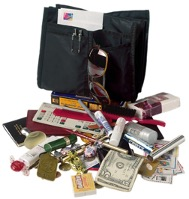
\includegraphics[width=0.5\textwidth]{Figures/Picture 2}
\caption{A Dictionary}
\end{figure}
\end{minipage}}%
\end{frame}
%
\section{Dictionaries}
\begin{frame}{Dictionaries}
\vfill
\begin{itemize}
	\item In Python, a dictionary is a mapping between a set of indices (\textit{keys}) and a set of \textit{values}\\
		\qquad $\rightarrow$ Items in a dictionary are \textcolor{red}{key-value pairs}
	\item Dictionaries are amongst the most powerful data collectors
	\item Dictionaries are also known as \textit{hash tables} or \textit{associative arrays}\\
		\qquad $\rightarrow$ They use a hash function for super-fast indexing of the keys
	\item Keys can't be any Python data type\\
		\qquad $\rightarrow$ Because keys are used for \textcolor{red}{indexing}, they should be \textcolor{red}{immutable}\\
		\qquad $\rightarrow$ Mutable objects do not support hashing\\
		\qquad $\rightarrow$ Common data types include strings and numbers
	\item Values can be any Python data type\\
		\qquad $\rightarrow$ Values can be \textcolor{red}{mutable} or \textcolor{red}{immutable}
\end{itemize}
\vfill
\end{frame}
%
\subsection{Creating a Dictionary}
\begin{frame}
\vfill
There are two ways for creating a dictionary:
\vfill
\begin{enumerate}
	\item Step-by-step
\end{enumerate}
\begin{table}[]
\begin{flushleft}
\begin{tabular}{ll}
\texttt{>{}>{}> d1 = dict()} & \# or \texttt{d1 = \{\}}, i.e., empty dictionary \\
\texttt{>{}>{}> d1['money'] = 12} &  \# add item\\
\texttt{>{}>{}> d1['candy'] = 3} &  \# add item\\
\texttt{>{}>{}> d1['tissues'] = 75} &  \# add item\\
\texttt{>{}>{}> print(d1)} &  \\
\texttt{\{'money': 12, 'candy': 3, 'tissues': 75\}} &  \\
\end{tabular}
\end{flushleft}
\end{table}
\vfill
\begin{enumerate}[2]
	\item All-at-once
\end{enumerate}
\begin{table}[]
\begin{flushleft}
\begin{tabular}{ll}
\texttt{>{}>{}> d2 = \{'money': 12, 'candy': 3, 'tissues': 75\}} &  \\
\texttt{>{}>{}> print(d2)} &  \\
\texttt{\{'money': 12, 'candy': 3, 'tissues': 75\}} &  \\
\end{tabular}
\end{flushleft}
\end{table}
\vfill
\end{frame}
%
\subsection{Indexing and Manipulating a Dictionary}
\begin{frame}
\vfill
\begin{itemize}
	\item Dictionary Query
\end{itemize}
\begin{table}[]
\begin{flushleft}
\begin{tabular}{ll}
\texttt{>{}>{}> d = \{'money': 12, 'candy': 3, 'tissues': 75\}} &  \\
\texttt{>{}>{}> print(d['money'])} & \\
\texttt{12} &  \\
\end{tabular}
\end{flushleft}
\end{table}
\begin{itemize}
	\item Update the Dictionary
\end{itemize}
\begin{table}[]
\begin{flushleft}
\begin{tabular}{ll}
\texttt{>{}>{}> d['candy'] = d['candy'] + 1} &  \\
\texttt{>{}>{}> print(d)} & \\
\texttt{\{'money': 12, 'candy': 4, 'tissues': 75\}} &  \\
\end{tabular}
\end{flushleft}
\end{table}
\vfill
\begin{itemize}
	\item Add New Items to the Dictionary
\end{itemize}
\begin{table}[]
\begin{flushleft}
\begin{tabular}{ll}
\texttt{>{}>{}> d['pen'] = 2} &  \\
\texttt{>{}>{}> print(d)} & \\
\texttt{\{'money': 12, 'candy': 4, 'tissues': 75, 'pen': 2\}} &  \\
\end{tabular}
\end{flushleft}
\end{table}
\vfill
\begin{itemize}
	\item Delete Items from the Dictionary
\end{itemize}
\begin{table}[]
\begin{flushleft}
\begin{tabular}{ll}
\texttt{>{}>{}> del(d['money'])} &  \# \texttt{del} works on lists too...\\
\texttt{>{}>{}> print(d)} & \\
\texttt{\{'candy': 4, 'tissues': 75, 'pen': 2\}} &  \\
\end{tabular}
\end{flushleft}
\end{table}
\end{frame}
%
\begin{frame}
\vfill
\begin{block}{Warning}
If the index is not a key in the dictionary, Python raises a dedicated \textcolor{red}{KeyError} error.
\end{block}
\begin{table}[]
\begin{flushleft}
\begin{tabular}{ll}
\texttt{>{}>{}> d = \{'money': 12, 'candy': 3, 'tissues': 75\}} &  \\
\texttt{>{}>{}> print(d['hello'])} & \\
\texttt{-{}-{}-{}-{}-{}-{}-{}-{}-{}-{}-{}-{}-{}-{}-{}-{}-{}-{}-{}-{}-{}-{}-{}-{}-{}-{}-{}-{}-{}-{}-{}-{}-{}-{}-{}-{}-{}-{}-{}-{}-{}-{}-{}-{}-{}-{}-{}-{}-{}-{}-{}-{}-{}-{}-{}-{}-{}-{}-{}-{}-{}-{}-{}-{}-{}-{}-{}-{}-{}-{}-{}-{}-{}-{}-{}} &  \\
\texttt{\textcolor{red}{KeyError} \ \ \ \ \ \ \ \ \ \ \ \ \ \ \ \ \ \ \ \ \ \ \ \ \ \ \ \ \ \ \ \ \ Traceback (most recent call last)} &  \\
...[truncated output] &  \\
...[truncated output] &  \\
\texttt{\textcolor{red}{KeyError}: 'hello'} &  \\
\end{tabular}
\end{flushleft}
\end{table}
\vfill
\end{frame}
%
\begin{frame}
\vfill
\begin{block}{Warning}
The \texttt{in} operator behaves differently with respect to lists and strings:
\begin{itemize}
	\item For offset-indexed sequences (e.g., strings and lists), \texttt{x in y} checks whether \texttt{x} is an item in the sequence \texttt{y}
	\item For dictionaries, \texttt{x in y} checks whether \texttt{x} \textit{is a key} of the dictionary \texttt{y}
\end{itemize}
\end{block}
\begin{table}[]
\begin{flushleft}
\begin{tabular}{ll}
\texttt{>{}>{}> L = [4, 6, 'hello', 7]} &  \# a list\\
\texttt{>{}>{}> 7 in L} & \\
\texttt{True} &  \\
\texttt{>{}>{}> s = 'coding with python'} &  \# a string\\
\texttt{>{}>{}> 'p' in s} & \\
\texttt{True} &  \\
\texttt{>{}>{}> d = \{'money': 12, 'candy': 3, 'tissues': 75\}} &  \# a dict\\
\texttt{>{}>{}> 'hello' in d} & \\
\texttt{False} &  \\
\texttt{>{}>{}> 'money' in d} & \\
\texttt{True} &  \\
\end{tabular}
\end{flushleft}
\end{table}
\vfill
\end{frame}
%------------------------------------------------------------------------------
\section{Dict Methods}
\subsection{\texttt{dict.keys()}, \texttt{dict.items()} and \texttt{dict.values()}}
\begin{frame}{Dict Methods}
\vfill
\texttt{dict.keys()} returns a \textit{view object}\footnote{View objects are dynamic overview on the dictionary's entries} containing all the keys of a dictionary.\\
You can conveniently cast into a list, a more common and flexible data object.
\begin{table}[]
\begin{flushleft}
\begin{tabular}{ll}
\texttt{>{}>{}> dishes = \{'eggs': 2, 'sausage': 1,} &   \\
\texttt{\qquad 'bacon': 1, 'spam': 500\}} &   \\
\texttt{>{}>{}> k = dishes.keys()} &   \# a view object (list-like)\\
\texttt{>{}>{}> print(k)} &   \\
\texttt{dict\_keys(['eggs', 'sausage', 'bacon', 'spam'])} &   \\
\texttt{>{}>{}> k = list(k)} &   \# a proper list \\
\texttt{>{}>{}> print(k)} &   \\
\texttt{['eggs', 'sausage', 'bacon', 'spam']} &   \\
\end{tabular}
\end{flushleft}
\end{table}
\begin{block}{Warning}
Dictionaries keep their items in the same order they were introduced\footnote{In Python 3.6 and earlier, dictionaries are fully unordered.}: \texttt{keys}, \texttt{values} and \texttt{items} (more on the latter later) are ordered according to this rule.
\end{block}
\vfill
\end{frame}
%
\begin{frame}
\vfill
\texttt{dict.values()} returns a \textit{view object} containing all the values of a dictionary.\\
\texttt{dict.items()} returns a \textit{view object} containing all the key-value pairs of a dictionary.\\
You can conveniently cast into a list, a more common and flexible data object.
\begin{table}[]
\begin{flushleft}
\begin{tabular}{ll}
\texttt{>{}>{}> dishes = \{'eggs': 2, 'sausage': 1,} &   \\
\texttt{\qquad 'bacon': 1, 'spam': 500\}} &   \\
\texttt{>{}>{}> v = dishes.values()} &   \# a view object (list-like) \\
\texttt{>{}>{}> v = list(v)} &   \# a proper list \\
\texttt{>{}>{}> print(v)} &   \\
\texttt{[2, 1, 1, 500]} &   \\
\texttt{>{}>{}> i = dishes.items()} &   \# a view object (list-like) \\
\texttt{>{}>{}> i = list(i)} &   \# a list of key-value tuples \\
\texttt{>{}>{}> print(i)} &   \\
\texttt{[('eggs', 2), ('sausage', 1),} &   \\
\texttt{\qquad ('bacon', 1), ('spam', 500)]} &   \\
\end{tabular}
\end{flushleft}
\end{table}
\vfill
\end{frame}
%
\subsection{\texttt{dict.get()}}
\begin{frame}
\vfill
\texttt{dict.get(key, [x])} returns the value for \texttt{key}. If \texttt{key} is not found, returns \texttt{x}. If \texttt{x} is not given, it defaults to \texttt{None}.
\begin{table}[]
\begin{flushleft}
\begin{tabular}{ll}
\texttt{>{}>{}> dishes = \{'eggs': 2, 'sausage': 1,} &   \\
\texttt{\qquad 'bacon': 1, 'spam': 500\}} &   \\
\texttt{>{}>{}> v = dishes.get('eggs', 10)} &   \# \texttt{'eggs'} exists in \texttt{dishes} \\
\texttt{>{}>{}> print(v)} &   \\
\texttt{2} &   \\
\texttt{>{}>{}> v = dishes.get('water', 10)} &   \# \texttt{'water'} does not exist in \texttt{dishes} \\
\texttt{>{}>{}> print(v)} &   \\
\texttt{10} &   \\
\end{tabular}
\end{flushleft}
\end{table}
\begin{block}{Note}
Since \texttt{dict.get()} relies on a default value if \texttt{key} is not found, it will never raise a \texttt{KeyError}.
\end{block}
\vfill
\end{frame}
%
\begin{frame}
\vfill
\begin{block}{Hint}
Pattern of usage: check whether a key is already in a dictionary and assuming a default value if the key is not there.
\end{block}
\begin{table}[]
\begin{flushleft}
\begin{tabular}{ll}
\texttt{>{}>{}> dishes = \{'eggs': 2, 'sausage': 1,} &   \\
\texttt{\qquad 'bacon': 1, 'spam': 500\}} &   \\
\# \texttt{'eggs'} exists in \texttt{dishes}, so we take its value and add + 1 &   \\
\texttt{>{}>{}> dishes['eggs'] = dishes.get('eggs', 0) + 1} &   \\
\texttt{>{}>{}> print(dishes)} &   \\
\texttt{dishes = \{'eggs': 3, 'sausage': 1,} &   \\
\texttt{\qquad 'bacon': 1, 'spam': 500\}} &   \\
\# \texttt{'water'} does not exists in \texttt{dishes} &   \\
\# so we plug the default value 0 and add + 1 &   \\
\texttt{>{}>{}> dishes['water'] = dishes.get('water', 0) + 1} &   \\
\texttt{>{}>{}> print(dishes)} &   \\
\texttt{dishes = \{'eggs': 3, 'sausage': 1,} &   \\
\texttt{\qquad 'bacon': 1, 'spam': 500, 'water': 1\}} &   \\
\end{tabular}
\end{flushleft}
\end{table}
\vfill
\end{frame}
%
\begin{frame}
\vfill
\texttt{dict.get()} explained:
\vfill
Let \texttt{d} be a dictionary. Saying\\
\texttt{v = d.get(k, x)}\\
is a shortcut for:
\begin{table}[]
\begin{flushleft}
\begin{tabular}{ll}
\texttt{if k in d:} &   \\
\texttt{\qquad v = d[k]} &   \\
\texttt{else:} &  \\
\texttt{\qquad v = x} &   \\
\end{tabular}
\end{flushleft}
\end{table}
\vfill
Similarly, saying\\
\texttt{d[k] = d.get(k, x) + y}\\
is a shortcut for:
\begin{table}[]
\begin{flushleft}
\begin{tabular}{ll}
\texttt{if k in d:} &   \\
\texttt{\qquad d[k] = d[k] + y} &   \\
\texttt{else:} &  \\
\texttt{\qquad d[k] = x + y} &   \\
\end{tabular}
\end{flushleft}
\end{table}
\vfill
\end{frame}
%
\subsection{\texttt{dict.clear()}}
\begin{frame}
\vfill
\texttt{dict.clear()} deletes all items from a dictionary.\\
\begin{table}[]
\begin{flushleft}
\begin{tabular}{ll}
\texttt{>{}>{}> dishes = \{'eggs': 2, 'sausage': 1,} &   \\
\texttt{\qquad 'bacon': 1, 'spam': 500\}} &   \\
\texttt{>{}>{}> dishes.clear()} &   \\
\texttt{>{}>{}> print(dishes)} &   \\
\texttt{\{\}} & \# an empty dictionary  \\
%\texttt{>{}>{}> dishes = \{'eggs': 2, 'sausage': 1,} &   \\
%\texttt{\qquad 'bacon': 1, 'spam': 500\}} &   \\
%\texttt{>{}>{}> v = dishes.pop('sausage')} &   \\
%\texttt{>{}>{}> print(dishes)} &   \\
%\texttt{\{'eggs': 2, 'bacon': 1, 'spam': 500\}} &   \\
\end{tabular}
\end{flushleft}
\end{table}
\begin{block}{Note}
There is a strong analogy with lists:
\begin{itemize}
%	\item \texttt{pop()} also returns the value when called on a list;
	\item \texttt{clear()} also works on lists (same effect $\rightarrow$ empty list).
\end{itemize}
\end{block}
\vfill
\end{frame}
%
\subsection{\texttt{dict.pop()}}
\begin{frame}
\vfill
%\texttt{dict.clear()} deletes all items from a dictionary.\\
\texttt{dict.pop(key)} deletes the dictionary entry corresponding to the key \texttt{key} and returns its value.\\
\begin{table}[]
\begin{flushleft}
\begin{tabular}{ll}
\texttt{>{}>{}> dishes = \{'eggs': 2, 'sausage': 1,} &   \\
\texttt{\qquad 'bacon': 1, 'spam': 500\}} &   \\
\texttt{>{}>{}> v = dishes.pop('sausage')} &   \\
\texttt{>{}>{}> print(dishes)} &   \\
\texttt{\{'eggs': 2, 'bacon': 1, 'spam': 500\}} &   \\
\texttt{>{}>{}> print(v)} &   \\
\texttt{1} &  \# former value for \texttt{'sausage'} \\
\end{tabular}
\end{flushleft}
\end{table}
\begin{block}{Note}
There is a strong analogy with lists:
\begin{itemize}
	\item \texttt{pop()} also returns the value when called on a list;
%	\item \texttt{clear()} also works on lists (same effect $\rightarrow$ empty list).
\end{itemize}
\end{block}
\vfill
\end{frame}
%
\subsection{\texttt{dict.update()}}
\begin{frame}
\vfill
\texttt{dict.update(other\_dict)} updates the dictionary \texttt{dict} with the key-value pairs from \texttt{other\_dict}, overwriting existing keys.\\
\begin{table}[]
\begin{flushleft}
\begin{tabular}{ll}
\texttt{>{}>{}> d1=\{1: 10, 2: 20\}} &   \\
\texttt{>{}>{}> d2=\{3: 30, 4: 40\}} &   \\
\texttt{>{}>{}> d1.update(d2)} &   \\
\texttt{>{}>{}> print(d1)} &   \\
\texttt{\{1: 10, 2: 20, 3: 30, 4: 40\}} & \# \texttt{d1} is modified in-place, \texttt{d2} is unchanged\\
%\texttt{>{}>{}> d1=\{1: 10, 2: 20\}} &   \\
%\texttt{>{}>{}> d2=\{3: 30, 2: 40\}} &  \# we have an overlapping key (i.e., \texttt{2}) \\
%\texttt{>{}>{}> d1.update(d2)} &   \\
%\texttt{>{}>{}> print(d1)} &   \\
%\texttt{\{1: 10, 2: 40, 3: 30\}} & \# the value associated to key \texttt{2} is taken from \texttt{d2} \\
\end{tabular}
\end{flushleft}
\end{table}
\begin{block}{Warning}
If a key exists both \texttt{dict} and \texttt{other\_dict}, the key-value pair in \texttt{other\_dict} overwrites the one in \texttt{dict}.
\end{block}
\vspace{-0.3cm}
\begin{table}[]
\begin{flushleft}
\begin{tabular}{ll}
%\texttt{>{}>{}> d1=\{1: 10, 2: 20\}} &   \\
%\texttt{>{}>{}> d2=\{3: 30, 4: 40\}} &   \\
%\texttt{>{}>{}> d1.update(d2)} &   \\
%\texttt{>{}>{}> print(d1)} &   \\
%\texttt{\{1: 10, 2: 20, 3: 30, 4: 40\}} & \# \texttt{d1} is modified in-place, \texttt{d2} is unchanged\\
\texttt{>{}>{}> d1=\{1: 10, 2: 20\}} &   \\
\texttt{>{}>{}> d2=\{3: 30, 2: 40\}} &  \# we have an overlapping key (i.e., \texttt{2}) \\
\texttt{>{}>{}> d1.update(d2)} &   \\
\texttt{>{}>{}> print(d1)} &   \\
\texttt{\{1: 10, 2: 40, 3: 30\}} & \# the value associated to key \texttt{2} is taken from \texttt{d2} \\
\end{tabular}
\end{flushleft}
\end{table}
\vfill
\end{frame}
%------------------------------------------------------------------------------
\section{Iterating over Dicts}
\begin{frame}{Iterating over Dicts}
You can iterate over a dictionary with a very simple \texttt{for} loop:
\begin{itemize}
	\item over its keys (way common)
	\item over its values (less common)
\end{itemize}
\begin{block}{Hint}
You can generate the sequence of keys and values with \texttt{dict.keys()} and \texttt{dict.values()}, respectively.
\end{block}
\begin{table}[]
\begin{flushleft}
\begin{tabular}{ll}
\texttt{dishes = \{'eggs': 2, 'sausage': 1,'bacon': 1, 'spam': 500\}} &   \\
\texttt{for k in dishes.keys():} &   \\
\texttt{\qquad print("Key is:", k, "and Value is:", dishes[k])} &   \\
\end{tabular}
\end{flushleft}
\end{table}
\begin{block}{Hint}
If you iterate over keys, it's trivial to have both key and value. If you iterate over values, it's not trivial to get the corresponding key.
\end{block}
\end{frame}
%
\begin{frame}
You can iterate \textcolor{red}{simultaneously} over keys and values of a dictionary with a very simple \texttt{for} loop.
\vfill
\begin{block}{Hint}
You can get the key-value pairs with \texttt{dict.items()}.
\end{block}
\vfill
\begin{table}[]
\begin{flushleft}
\begin{tabular}{ll}
\texttt{dishes = \{'eggs': 2, 'sausage': 1,'bacon': 1, 'spam': 500\}} &   \\
\texttt{for k, v in dishes.items():} &   \\
\texttt{\qquad print("Key is:", k, "and Value is:", v)} &   \\
\end{tabular}
\end{flushleft}
\end{table}
\vfill
What's going on here?
\begin{itemize}
	\item there are \textcolor{red}{two iteration variables}, namely \texttt{k} and \texttt{v}
	\item \texttt{dict.items()} generates a list of key-value pairs (tuple)
	\item the first loop variable, namely \texttt{k}, contains the key in the key-value pair
	\item the second loop variable, namely \texttt{v}, contains the corresponding value in the key-value pair
\end{itemize}
\end{frame}
%------------------------------------------------------------------------------
\section{Tuples}
\begin{frame}{Tuples}
Tuples, like lists, are \textcolor{red}{ordered collections} of items.\\
You can create a tuple by enclosing items in round brackets:
\begin{table}[]
\begin{flushleft}
\begin{tabular}{ll}
\texttt{>{}>{}> t1 = (90, 98, 95)} & \# homogeneous tuple  \\
\texttt{>{}>{}> t2 = (90, 'hello', 95, [1, 2])} & \# heterogeneous tuple  \\
\texttt{>{}>{}> t3 = ()} & \# empty tuple  \\
\end{tabular}
\end{flushleft}
\end{table}
or, you can omit the parenthesis altogether\footnote{This is called \textit{tuple packing}.}
\begin{table}[]
\begin{flushleft}
\begin{tabular}{ll}
\texttt{>{}>{}> t1 = 90, 98, 95} & \# homogeneous tuple  \\
\texttt{>{}>{}> t2 = 90, 'hello', 95, [1, 2]} & \# heterogeneous tuple  \\
\end{tabular}
\end{flushleft}
\end{table}
\begin{block}{Warning}
When you create a singleton tuple, you must include a tailing comma!
\end{block}
\begin{table}[]
\begin{flushleft}
\begin{tabular}{ll}
\texttt{>{}>{}> t = (90)} & \# \texttt{type(t)} yields \texttt{'int'}  \\
\texttt{>{}>{}> t = (90,)} & \# now we have a 1-element tuple \\
\end{tabular}
\end{flushleft}
\end{table}
\end{frame}
%
\begin{frame}
\vfill
Tuples (and lists) can also be \textit{unpacked}\footnote{Unpacking is when you assign values from a tuple/list to a sequence of variables.}.
\vfill
\begin{table}[]
\begin{flushleft}
\begin{tabular}{ll}
\texttt{>{}>{}> t = (90, 0, 'hello')} & \\
\texttt{>{}>{}> a, b, c = t} &  \# unpacking syntax\\
\end{tabular}
\end{flushleft}
\end{table}
\vfill
which is basically the same as doing
\begin{table}[]
\begin{flushleft}
\begin{tabular}{ll}
\texttt{>{}>{}> a = t[0]} & \\
\texttt{>{}>{}> b = t[1]} & \\
\texttt{>{}>{}> c = t[2]} & \\
\end{tabular}
\end{flushleft}
\end{table}
\vfill
and therefore we will have:
\begin{table}[]
\begin{flushleft}
\begin{tabular}{ll}
\texttt{a} $\rightarrow$ \texttt{90} & \\
\texttt{b} $\rightarrow$ \texttt{0} & \\
\texttt{c} $\rightarrow$ \texttt{'hello'} & \\
\end{tabular}
\end{flushleft}
\end{table}
\vfill
\end{frame}
%
\begin{frame}
\vfill
Tuples support all of the common operations we have for lists, notably:
\begin{itemize}
	\item indexing\\
	\quad\texttt{t=(98, 7, 'hello')} \qquad \texttt{t[1]} yields \texttt{7} \\
	\item slicing\\
	\quad\texttt{t=(98, 7, 'hello', 'world')} \qquad \texttt{t[1:3]} yields \texttt{(7, 'hello')} \\
	\item the \texttt{+} operator for concatenation\\
	\quad\texttt{t1=(98, 7)} and \texttt{t2=('hello',)} \qquad \texttt{t1+t2} yields \texttt{(98, 7, 'hello')} \\
	\item the \texttt{*} operator for replication\\
	\quad\texttt{t=(98, 7)} \qquad \texttt{t*3} yields \texttt{(98, 7, 98, 7, 98, 7)} \\
	\item the \texttt{in} (and \texttt{not in}) operator for membership checking\\
	\quad\texttt{t=(98, 7)} \qquad \texttt{'hello' in t} yields \texttt{False} \\
	\item the \texttt{len()} function to calculate the length of a tuple
\end{itemize}
\vfill
And you can also iterate over tuples, e.g. via \texttt{for} loops:
\begin{table}[]
\begin{flushleft}
\begin{tabular}{ll}
\texttt{t = (98, 7, 'hello')} & \\
\texttt{for item in t:} & \\
\texttt{\qquad print(item)} & \\
\end{tabular}
\end{flushleft}
\end{table}
\vfill
\end{frame}
%
\begin{frame}
\vfill
Yet, \textcolor{red}{tuples are immutable}, whereas \textcolor{red}{lists are mutable}.
\begin{table}[]
\begin{flushleft}
\begin{tabular}{ll}
\texttt{>{}>{}> t = (98, 7, 'hello')} & \\
\texttt{>{}>{}> t[-1] = 'python'} & \\
\texttt{-{}-{}-{}-{}-{}-{}-{}-{}-{}-{}-{}-{}-{}-{}-{}-{}-{}-{}-{}-{}-{}-{}-{}-{}-{}-{}-{}-{}-{}-{}-{}-{}-{}-{}-{}-{}-{}-{}-{}-{}-{}-{}-{}-{}-{}-{}-{}-{}-{}-{}-{}-{}-{}-{}-{}-{}-{}-{}-{}-{}-{}-{}-{}-{}-{}-{}-{}-{}-{}-{}-{}-{}-{}-{}-{}} &  \\
\texttt{\textcolor{red}{TypeError}: 'tuple' object does not support item assignment} &  \\
\end{tabular}
\end{flushleft}
\end{table}
\vfill
So you cannot change a tuple, just like you cannot change a string. Workarounds:
\begin{itemize}
	\item create a new tuple that contains the manipulation of the original tuple
	\item cast tuple to list, change the list, cast list to tuple
\end{itemize}
\vfill
As the latter is concerned:
\begin{table}[]
\begin{flushleft}
\begin{tabular}{ll}
\texttt{>{}>{}> t = (98, 7, 'hello')} & \# \texttt{t} is a tuple\\
\texttt{>{}>{}> L = list(t)} & \# from tuple to list\\
\texttt{>{}>{}> print(L)} & \\
\texttt{[98, 7, 'hello']} & \\
\texttt{>{}>{}> L.append('python')} & \# do some manipulations\\
\texttt{>{}>{}> t = tuple(L)} & \# from list to tuple\\
\texttt{>{}>{}> print(t)} & \\
\texttt{(98, 7, 'hello', 'python')} & \\
\end{tabular}
\end{flushleft}
\end{table}
\vfill
\end{frame}
%------------------------------------------------------------------------------
% \section{Exercises}
% \begin{frame}{Exercises}
% \textcolor{red}{Exercise \#1: Names histogram.}\\
% \vspace{0.4cm}
% Write a function called \texttt{namehist()} that:
% \begin{itemize}
% 	\item takes as input a list \texttt{names}
% 	\item returns a dictionary containing the number of times each name appears in \texttt{names}
% \end{itemize}
% %\textcolor{red}{Exercise \#1: count the number of times each name appears in the list \texttt{names}.}
% %\begin{table}[]
% %\begin{flushleft}
% %\begin{tabular}{ll}
% %\texttt{names = ['irene', 'mattia', 'giorgio', 'irene', } &   \\
% %\texttt{\qquad 'giorgio', 'alessio', 'carlo', 'irene']} &   \\
% %\texttt{counts = dict()} &   \\
% %\texttt{for name in names:} &   \\
% %\texttt{\qquad if name in counts:} &   \\
% %\texttt{\qquad\qquad counts[name] += 1} &   \\
% %\texttt{\qquad else:} &   \\
% %\texttt{\qquad\qquad counts[name] = 1} &   \\
% %\texttt{print(counts)} &   \\
% %\end{tabular}
% %\end{flushleft}
% %\end{table}
% You can assume, for example:\\
% \texttt{names = ['irene', 'mattia', 'giorgio', 'irene', }\\
% \texttt{\qquad 'giorgio', 'alessio', 'carlo', 'irene']}
% \vfill
% \begin{block}{Note}
% One common use of dictionaries is counting how many times we have something.
% \end{block}
% \end{frame}
% %
% \begin{frame}
% \textcolor{red}{Exercise \#2: Inverter.}\\
% \vspace{0.4cm}
% Write a function called \texttt{inverter()} that:
% \begin{itemize}
% 	\item takes as input a dictionary \texttt{d}
% 	\item returns a new dictionary where values and keys are swapped (i.e., keys in \texttt{d} are values in the new dictionary and values in \texttt{d} are keys in the new dictionary).
% \end{itemize}
% \vspace{0.4cm}
% You can assume, for example:\\
% \texttt{d = \{1: "Jan", 2: "Feb", 3: "Mar", 4: "Apr", 5: "May", }\\
% \texttt{\qquad 6: "Jun", 7: "Jul", 8: "Aug", 9: "Sep", }\\
% \texttt{\qquad 10: "Oct", 11: "Nov", 12: "Dec"\} }
% \end{frame}
% %
% \begin{frame}
% \textcolor{red}{Exercise \#3: Dict of Squares.}\\
% \vspace{0.4cm}
% Write a function called \texttt{dictsquares()} that:
% \begin{itemize}
% 	\item takes an integer number \texttt{n}
% 	\item returns a dictionary where the keys are numbers between $1$ and $n$ (both included) and the values are the square of keys.
% \end{itemize}
% \vspace{0.4cm}
% Caveats:
% \begin{itemize}
% 	\item if $n < 0$, then the function must return an empty dictionary
% 	\item if \texttt{n} is a float, then the function must return an empty dictionary
% \end{itemize}
% \vspace{0.4cm}
% \begin{block}{Hint}
% Use the \texttt{type()} function to assess the type of a variable.
% \end{block}
% \end{frame}
% %
% \begin{frame}
% \textcolor{red}{Exercise \#4: List Mapper.}\\
% \vspace{0.4cm}
% Write a function called \texttt{listMapper()} that:
% \begin{itemize}
% 	\item takes as input two lists \texttt{L1} and \texttt{L2}
% 	\item returns a dictionary where the keys are the items from \texttt{L1} and the values are the items from \texttt{L2}
% \end{itemize}
% \vspace{0.4cm}
% You can assume \texttt{L1} and \texttt{L2} having the same length.\\
% \vspace{0.4cm}
% You can assume, for example:\\
% \texttt{keys = ['red', 'green', 'blue']}\\
% \texttt{values = ['\#FF0000','\#008000', '\#0000FF']}
% \end{frame}
% %
% \begin{frame}
% \textcolor{red}{Exercise \#5: Minimum \& Maximum Value.}\\
% \vspace{0.4cm}
% Write a function called \texttt{minMaxVal()} that:
% \begin{itemize}
% 	\item takes as input a dictionary \texttt{d} with numerical values
% 	\item returns the minimum and maximum value across \texttt{d}
% \end{itemize}
% \vspace{0.4cm}
% You can assume, for example:\\
% \texttt{d = \{'x':500, 'y':5874, 'z': 560\}}
% \vspace{0.4cm}
% \begin{block}{Hint}
% Use the \texttt{min()} and \texttt{max()} functions to calculate the minimum and maximum value. They accept any iterable sequence as input (e.g., lists and tuples).
% \end{block}
% \end{frame}
% %
% \begin{frame}
% \textcolor{red}{Exercise \#6: Adder Combiner.}\\
% \vspace{0.4cm}
% Write a function called \texttt{adder()} that:
% \begin{itemize}
% 	\item takes as input two dictionaries \texttt{d1} and \texttt{d2} with numerical values
% 	\item returns a new dictionary by adding the corresponding values for common keys in \texttt{d1} and \texttt{d2}. Keys that exist in either \texttt{d1} or \texttt{d2} should have their values untouched.
% \end{itemize}
% \vspace{0.4cm}
% You can assume, for example:\\
% \texttt{d1 = \{'a': 100, 'b': 200, 'c':300\}}\\
% \texttt{d2 = \{'a': 300, 'b': 200, 'd':400\}}
% \end{frame}
%------------------------------------------------------------------------------
\section{Sets}
\begin{frame}{Sets}
	\vfill
A set is an unordered (unindexed) collection of items with no repetitions.
	\vfill
	You can create an empty set thanks to the \texttt{set()} function.
	\vfill
	And you can create a non-empty set thanks to the \texttt{set()} function or curly brackets.
\vfill
\begin{table}[]
	\begin{flushleft}
	\begin{tabular}{ll}
	\# empty set& \\
	\texttt{>{}>{}> s1 = set()} & \\
	\# non-empty set with curly brackets & \\
	\texttt{>{}>{}> s2 = \{'a', 1\}} & \\
	\# non-empty set with \texttt{set()}\\
	\texttt{>{}>{}> s3 = set(['a', 1])} & \\
	\end{tabular}
	\end{flushleft}
\end{table}
\vfill
\begin{block}{Warning}
	To not confuse the curly brackets to create dicts with the curly brackets to create sets.
	\end{block}
	\vfill
\end{frame}
%
\begin{frame}
\vfill
A set can contain only hashable items, notably:
\begin{itemize}
	\item numbers
	\item strings
	\item tuples only if they do not contain mutable objects
\end{itemize}
and in no way they can contain mutable objects, notably:
\begin{itemize}
	\item dictionaries
	\item lists
	\item tuples that contain mutable objects
\end{itemize}
\vfill
In Python, the majority of immutable objects are also hashable.
\vfill
\end{frame}
%
\begin{frame}
\vfill
Hashing is a concept in computer science which is used to create high performance, pseudo random access data structures where large amount of data is to be stored and accessed quickly.
\vfill
The hash of some data is deterministic by design and will never change if the data does not change
\begin{itemize}
	\item this is why mutable objects are not hashable ...
\end{itemize}
\vfill
Also, matching the hashes of the data is usually faster than matching the data itself.
\vfill
Sets and dictionary keys use hashing for fast access and look-up.
\begin{block}{Example: \texttt{if x in X}}
If \texttt{X} is a list, then Python scans the entire list until \texttt{x} is found: $\mathcal{O}(n)$\\
If \texttt{X} is a dictionary or set, \textit{hash(}\texttt{x}\textit{)} gives the position in memory: $\mathcal{O}(1)$.
\end{block}
\vfill
\end{frame}
%
\begin{frame}
	\vfill
Functions for sets:
\begin{itemize}
	\item membership\\
	\quad\texttt{x in S}
	\item the \texttt{len(s)} function to calculate the cardinality (size) of a set \texttt{s}
\end{itemize}
Operations between sets:
\begin{itemize}
	\item union (new set with elements in either \texttt{s1} or \texttt{s2})\\
	\quad\texttt{s1 | s2} \qquad or \qquad \texttt{s1.union(s2)}
	\item intersection (new set with elements in both \texttt{s1} and \texttt{s2})\\
	\quad\texttt{s1 \& s2} \qquad or \qquad \texttt{s1.intersection(s2)}
	\item difference (new set with elements in \texttt{s1} but not in \texttt{s2})\\
	\quad\texttt{s1 - s2} \qquad or \qquad \texttt{s1.difference(s2)}
	\item symmetric difference (new set with elements in \texttt{s1} or \texttt{s2}, but not both)\\
	\quad\texttt{s1 \^{} s2} \qquad or \qquad \texttt{s1.symmetric\_difference(s2)}
\end{itemize}
\vfill
\begin{block}{Note}
Set operations yield a brand new set.
\end{block}
\vfill
\end{frame}
%
\begin{frame}
	\vfill
Set methods:
\begin{itemize}
	\item \texttt{s.add(x)}\\
	\quad adds \texttt{x} to the set \texttt{s} (if \texttt{x} already in \texttt{s}, nothing happens)
	\item \texttt{s.remove(x)}\\
	\quad removes \texttt{x} from the set \texttt{s} (if \texttt{x} is not in \texttt{s}, a \texttt{KeyError} is raised)
	\item \texttt{s.discard(x)}\\
	\quad removes \texttt{x} from the set \texttt{s} (if \texttt{x} is not in \texttt{s}, nothing happens)
	\item \texttt{s.update(x)}\\
	\quad adds elements from \texttt{x} into the set \texttt{s} (\texttt{x} can be any iterable, e.g., list, tuple or another set)
	\item \texttt{s.clear()}\\
	\quad removes all elements from \texttt{s}
	\item \texttt{s.pop()}\\
	\quad removes (and returns) an arbitrary item from \texttt{s}
\end{itemize}
\vfill
\begin{block}{Note}
Set methods change the set in-place.
\end{block}
\vfill
\end{frame}
%------------------------------------------------------------------------------
\section{Recap on Collections}
\begin{frame}{Recap on Collections}
\vfill
\begin{itemize}
	\item \texttt{list} and \texttt{tuple} keep order; \texttt{set} and \texttt{dict} do not
	\item \texttt{dict} associates a key with a value; \texttt{set}, \texttt{tuple} and \texttt{list} contain just values
	\item \texttt{set} and \texttt{dict} keys only require items to be hashable; \texttt{list}, \texttt{tuples} and \texttt{dict} values do not
	\item \texttt{set} and \texttt{dict} keys forbid duplicates; \texttt{list}, \texttt{tuples} and \texttt{dict} values allow duplicates.
\end{itemize}
\vfill
Checking for membership inside a \texttt{set} or \texttt{dict} is super-fast thanks to hashing.\\
\texttt{tuple} and \texttt{list} require scanning the list/tuple until the element is found.
\vfill
\end{frame}
%------------------------------------------------------------------------------
%\section{References}
%\begin{frame}[allowframebreaks]{References}
%%\bibliographystyle{apacite}
%\printbibliography[heading=none]
%\end{frame}
\section{References}
\begin{frame}{References}
\begin{itemize}
	\item Guttag, J. V. (2013). \textit{Introduction to Computation and Programming using Python (Revised and Expanded Edition)}. MIT Press. [Sections 5.1, 5.4 \& 5.5]
	\item Downey, A. (2015). \textit{Think Python}. Green Tea Press ed. 2nd. [Chapters 11 \& 12]
	\item \url{https://docs.python.org/3/library/stdtypes.html\#dict}
	\item \url{https://docs.python.org/3/library/stdtypes.html\#typesseq-common}
\end{itemize}
\end{frame}
%------------------------------------------------------------------------------
\section{Acknowledgments}
\begin{frame}{Acknowledgments}
% \begin{itemize}
% 	\item Prof. Irene Finocchi (LUISS University)\\
% 	\quad \textit{Introduction to Computer Programming} Lecture Notes (2020-2021)
% \end{itemize}
\end{frame}
%------------------------------------------------------------------------------
%\subsection{Sites legais}
%\begin{frame}{Sites legais}
%  Want to know more? See!
%  \begin{itemize}
%    \item Browse in my page \url{http://www.ezefranca.com}.
%    \item Browse on BCC page \url{http://www.sp.senac.br/bcc}.
%    \item Thanks WriteLaTeX from Support! \url{http://www.writelatex.com}.
%  \end{itemize}
%
%\end{frame}
%------------------------------------------------------------------------------

% -----------------------------------------------------------------------------
\end{document}
%-----------------------------------------------Este comentario nunca aparecera
